% 
% Lecture Template for ME3050 -  Dynamics Modeling and Controls - Tennessee Technological University
%
% Spring 2020 - Summer 2020
% Tristan Hill, May 07, 2020
% Dyanmics Review - Topic 3 - Modeling Assumptions
%

\documentclass{beamer}                         % for presentation (has nav buttons at bottom)
%\documentclass[handout]{beamer}  % for handout 
\usepackage{beamerthemesplit}
\usepackage{amsmath}
\usepackage{listings}
\usepackage{multicol}

\beamertemplateballitem

\definecolor{TTUpurple}{rgb}{0.3098, 0.1607, 0.5176} % TTU Purple (primary)
\definecolor{TTUgold}{rgb}{1.0000, 0.8666, 0.0000} % TTU Gold (primary)

\setbeamercolor{palette primary}{bg=TTUpurple,fg=TTUgold}
\setbeamercolor{palette secondary}{bg=black,fg=TTUgold}
\setbeamercolor{palette tertiary}{bg=black,fg=TTUpurple}
\setbeamercolor{palette quaternary}{bg=TTUgold,fg=black}
\setbeamercolor{structure}{fg=TTUpurple} % itemize, enumerate, etc
\setbeamercolor{section in toc}{fg=TTUpurple} % TOC sections

%\usefonttheme{professionalfonts}

\newcommand{\Lagr}{\mathcal{L}} % lagrangian

\newcommand{\vspccc}{\vspace{6mm}\\} % large vertical space
\newcommand{\vspcc}{\vspace{4mm}\\}   % medium vertical space
\newcommand{\vspc}{\vspace{2mm}\\}     % small vertical space

\newcommand{\hspcccc}{\hspace{10mm}} % large horizontal space
\newcommand{\hspccc}{\hspace{6mm}} % large horizontal space
\newcommand{\hspcc}{\hspace{4mm}}   % medium horizontal space
\newcommand{\hspc}{\hspace{2mm}}     % small horizontal space


\author{ME3050 - Dynamics Modeling and Controls} % original formatting from Mike Renfro, September 21, 2004

\newcommand{\TNUM}{3\hspace{2mm}} % topic Number 
\newcommand{\topictitle}{Modeling Assumptions } % first line of title (used by beamer)
\newcommand{\sectiontitle}{Dynamics Review }% second line of the title of this presentation (used by TWH)

\title{\sectiontitle - \topictitle}

\date{May 29, 2020}

\begin{document}

\lstset{language=MATLAB,basicstyle=\ttfamily\small,showstringspaces=false}

\frame{\titlepage \center\textbf{Topic \TNUM - \topictitle}\vspace{5mm}\\}

% Section 0: Outline


\frame{

\large \textbf{Topic \TNUM - \topictitle} \vspace{3mm}\\

%Topics : \vspace{3mm}\\ % ' topics' are beamer 'sections' - TWH

\begin{itemize}
	\item Simplify Complex Systems\vspace{3mm}\\ % Section 1
	\item Increase Complexity Incrementally\vspace{3mm}\\% Section 2
	\item Solid Mechanics and Dynamics\vspace{3mm}\\ %Section 3
	\item Thermal and Fluid Systems \vspace{3mm}\\  %Section 4
	\item Electrical and Power Systems \vspace{3mm}\\  %Section 5
\end{itemize}
}

% Section 1:
\section{Simplify Complex Systems}

\frame{
\frametitle{Simplify Complex Systems}
\begin{multicols}{2}
Engineers encounter complex systems and these systems are difficult to model and analyze.  Analysis requires multiple steps or processes and modeling requires iteration. Typically, you cannot solve these complex problems in your head alone. \vspc

\includegraphics[scale=.15]{fanuc_robot.jpg}
\end{multicols}
{\tiny \hspace{60mm} Image: \href{https://en.wikipedia.org/wiki/Articulated_robot}{Wikipedia} }

}

% Section 2: 
\section{Increase Complexity Incrementally}

\frame{
\frametitle{Increase Complexity Incrementally}


Engineers model and analyze complex systems one piece at a time on a component level. \vspc

In system dynamics we study the behavior of complex systems by modeling the iterations and responses of the different components involved. Our models will start simple and build in complexity as the theory is presented. 

}

% Section 3: 
\section{Solid Mechanics and Dynamics}

\frame{
\frametitle{Solid Mechanics and Dynamics}

\begin{multicols}{2}
\begin{itemize}
\item Frictionless Sliding  ?
\item Pure Roll - No Slip 
\item Planar Motion \\
\end{itemize}

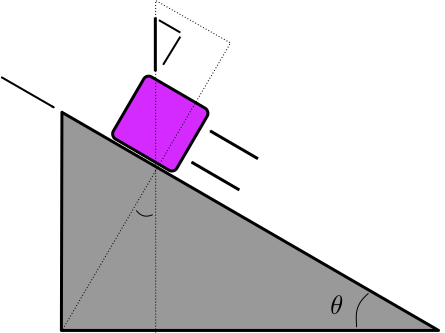
\includegraphics[scale=0.209]{sliding_block.png}
 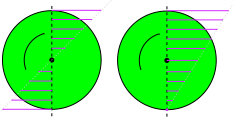
\includegraphics[scale=0.125]{pure_roll_no_slip.png} 
 \includegraphics[scale=0.17]{cartesian_3d.png}
\end{multicols}
{\tiny Image: TH\hspace{60mm} Images: TH, \href{https://en.wikipedia.org/wiki/Cartesian_coordinate_system}{Wikipedia} }

}

% Section 4:
\section{Thermal and Fluid Systems}

\frame{
\frametitle{Thermal and Fluid Systems}

\begin{itemize}
\item Viscous Boundary Layer
\item Insulated or Constant Flux Boundaries
\item Others?
\end{itemize}

}

% Section 5:
\section{Electrical and Power Systems}

\frame{
\frametitle{Electrical and Power Systems}

\begin{multicols}{2}
\begin{itemize}
\item No Heat Loss or Generation
\item Ideal Conductors
\item Zero Order System Behavior
\end{itemize}


\includegraphics[scale=.25]{rc_circuit.png}
\end{multicols}
{\hspace{60mm}\tiny Image: TH}
}
	
\end{document}



